\chapter{Project implementation}
The project is developed in Pandapower a, Python based, power system analysis tool aimed at automation of static and quasi-static analysis and optimization of balanced power systems \cite{pandapower}.\\
The network employed for these experiments is the network used in the paper \cite{gym-anm}; it consists of: one external grid, five buses, one transformer, four lines, three loads, two static generators and one \gls{DES} device.

\begin{figure}[h]
\centering
    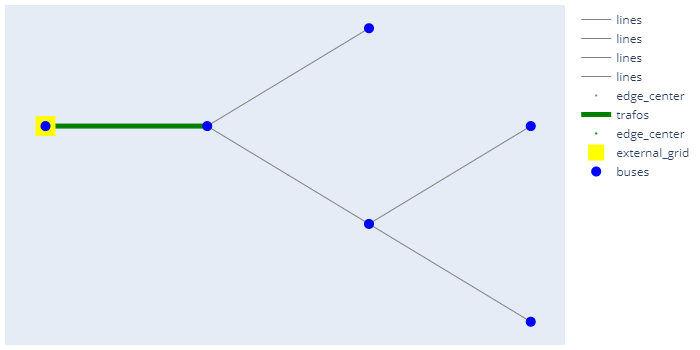
\includegraphics[width=.7\linewidth]{images/GYM-ANM/NETS/Gyn-anm network.png}
\caption{GYM-ANM network}
\label{fig:gym_anm_net}
\end{figure}

\noindent Following the paper, 3 situations are tested obtaining similar results:\\
\textbf{Situation 1} \\
    This situation (figure: \ref{fig:net_sit1}) characterises a windy night, when the consumption is low, the PV
    production null, and the wind production at it is near maximum. Due to the very low demand from the industrial load, the wind production must be curtailed to avoid an overheating of the transmission lines connecting
    buses 0 and 4.
    \begin{figure}[H]
    \centering
        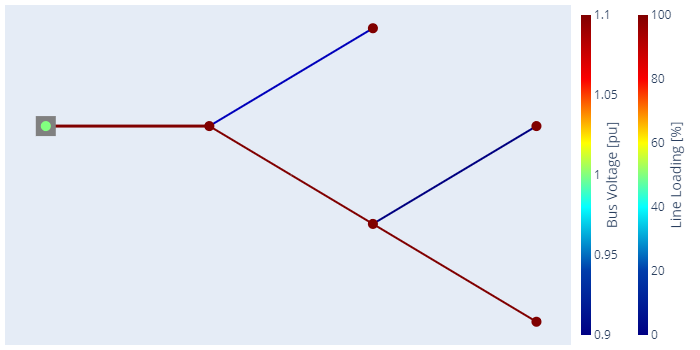
\includegraphics[width=.7\linewidth]{images/GYM-ANM/NETS/Gyn-anm network situation1.png}
    \caption[GYM-ANM network situation 1]{GYM-ANM network situation 1. Interactive image at the following \href{https://htmlpreview.github.io/?https://github.com/MauriVass/ThesisLiege/blob/master/Images/fig_case1.html}{link}}
    \label{fig:net_sit1}
    \end{figure}
    
\noindent \textbf{Situation 2} \\
    In this situation (figure: \ref{fig:net_sit2}), bus 5 is experiencing a substantial demand due to a large number
    of EVs being plugged-in at around the same time. This could happen in a large public EV charging garage. In the morning, workers of close-by companies would plug in their car after arriving at work and, in the evening, residents of the area would plug in their cars after getting home. In order to emphasise the problems arising from this large, localised demand, we assume that the other buses (3 and 4) inject or withdraw very little power into/from the network. During those periods of the day, the DES unit must provide enough power to ensure that the transmission path from bus 0 to bus 5 is not overrated, which would lead to an overheating of the line. For this to be possible, the agent must strategically plan ahead to ensure a sufficient charge level
    at the \gls{DES} unit.
    \begin{figure}[h]
    \centering
        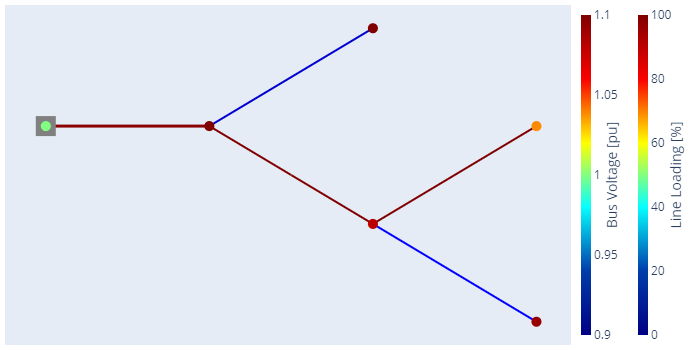
\includegraphics[width=.7\linewidth]{images/GYM-ANM/NETS/Gyn-anm network situation2.png}
    \caption[GYM-ANM network situation 2]{GYM-ANM network situation 2. Interactive image at the following \href{https://htmlpreview.github.io/?https://github.com/MauriVass/ThesisLiege/blob/master/Images/fig_case2.html}{link}}
    \label{fig:net_sit2}
    \end{figure}
    
\noindent \textbf{Situation 3} \\
    Situation (figure: \ref{fig:net_sit3}), represents a scenario that might occur in the middle of a sunny windy weekday. No one is home to consume the solar energy produced by residential PVs at bus 1 and the wind energy production exceeds the industrial demand at bus 2. In this case, both renewable generators should be
    adequately curtailed while again storing some extra energy to anticipate the EV late afternoon charging period, as depicted in Situation 2.
    \begin{figure}[h]
    \centering
        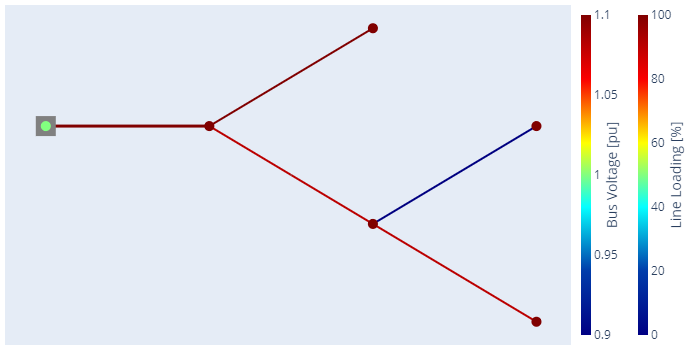
\includegraphics[width=.7\linewidth]{images/GYM-ANM/NETS/Gyn-anm network situation3.png}
    \caption[GYM-ANM network situation 3]{GYM-ANM network situation 3. Interactive image at the following \href{https://htmlpreview.github.io/?https://github.com/MauriVass/ThesisLiege/blob/master/Images/fig_case3.html}{link}}
    \label{fig:net_sit3}
    \end{figure}
    
\section{Generate dataset}
Pandapower allows running time series simulations of a network. When calling the time series function, a loop starts to iterate for each time step and the power flow of the network is calculated.\\
For this simulation, a time $\Delta t$ of 15 minutes if used for a temporal window of one year, in total of 35,040 time steps. To be compliant to Pandapower requirements, the time series must be passed to a controller that will change the network's devices values for each loop.\\
The results in this section are obtained with the following time series:

\begin{algorithm}[H]
\caption{Time series of active power \gls{P} for loads \gls{L} and generators \gls{G}}
\label{alg:timeseries}
\begin{algorithmic}[1]
\State $n\_timesteps = 365 * 24 * 4$

\LineComment{Loads active power}
\State $Load0\_p = cos(range(n\_timesteps))^2* rand(n\_timesteps)*4$
\State $Load1\_p = normal(7,0.5, size=n\_timesteps)$
\State $Load2\_p = normal(14,0.5, size=n\_timesteps)$

\LineComment{Generators active power}
\State $PVgen\_p = normal(4,0.5, size=n\_timesteps)$
\State $Windgen\_p = cos(range(n\_timesteps))^2*rand(n\_timesteps)*12$

%\end{small}
\end{algorithmic}
\end{algorithm}

After the simulation is run, some output values are exported as \emph{.xlsx} files and these constitute the dataset, the story of the network. These output values are:
\begin{itemize}
    \item loads active power in MW.
    \item buses voltage magnitude in \gls{pu}.
    \item the lines loading in percentages and the current in kA.
\end{itemize}

\begin{figure}[h]
    \centering
    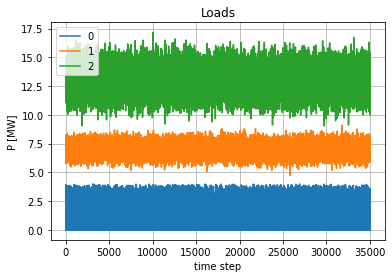
\includegraphics[width=.32\linewidth]{images/GYM-ANM/DATASET PLOTS/loads.png}
    \includegraphics[width=.32\linewidth]{images/GYM-ANM/DATASET PLOTS/VM.png}
    \includegraphics[width=.32\linewidth]{images/GYM-ANM/DATASET PLOTS/LL.png}
    \caption[GYM-ANM datasets]{Loads active power, buses voltage magnitude and line percentage loading}
    \label{fig:net_sit3}
\end{figure}
    
    
\section{Voltage lines forecasting}
\subsection{Splitting the dataset}
The aforementioned dataset is divided in training, validation and test set in 70, 20 and 10 percent respectively, without a random shuffle before the splitting. This has two main advantages:
\begin{enumerate}
    \item It ensures that chopping the data into windows of consecutive samples is still possible.
    \item It ensures that the validation/test results are more realistic, being evaluated on the data collected after the model was trained.
\end{enumerate}

\subsection{Normalization}
The data is normalised subtracting the mean and dividing by the standard deviation of each feature. The mean and standard deviation are computed using the training data so that the models have no access to the values in the validation and test sets.

\subsection{Windowing}
The training, validation and test sets are divided in windows to then fed to the neural network. \\
The main features of the windows are:
\begin{itemize}
    \item The width (number of time steps) of the input and label windows.
    \item The time offset between them.
    \item Which features are used as inputs, labels, or both.
\end{itemize}

The result are obtained using an input window of 12 time steps and an output window of 6 time steps. The offset is 1, this means that the predictions are from time step 13 to 18. The training features are:
\begin{algorithmic}
\State $[load0\_p, load1\_p, load2\_p, PVgen\_p, Wind gen\_p, L0, L1, L2, L3]$
\end{algorithmic}
and the label features are:
\begin{algorithmic}
\State $[L0, L1, L2, L3]$
\end{algorithmic}
where $Li$ is the loading in percentage of line $i$.

\begin{figure}[h]
    \centering
    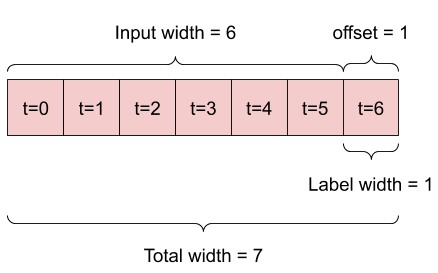
\includegraphics[width=.7\linewidth]{images/GYM-ANM/DATASET PLOTS/raw_window_1h.png}
    \caption[GYM-ANM datasets windowing]{Window visual representation for the input and output time steps \\
    TODO: add an image that shows the real situation (This is taken from Tensorflow website)}
    \label{fig:net_sit3}
\end{figure}

\subsection{Training}
The model used for training is an artificial neural network with two hidden layers with 128 and 64 neurons respectively.\\
The neural network is trained for 20 epochs with Adam optimizer and early stopping callback.

\begin{figure}[H]
    \centering
    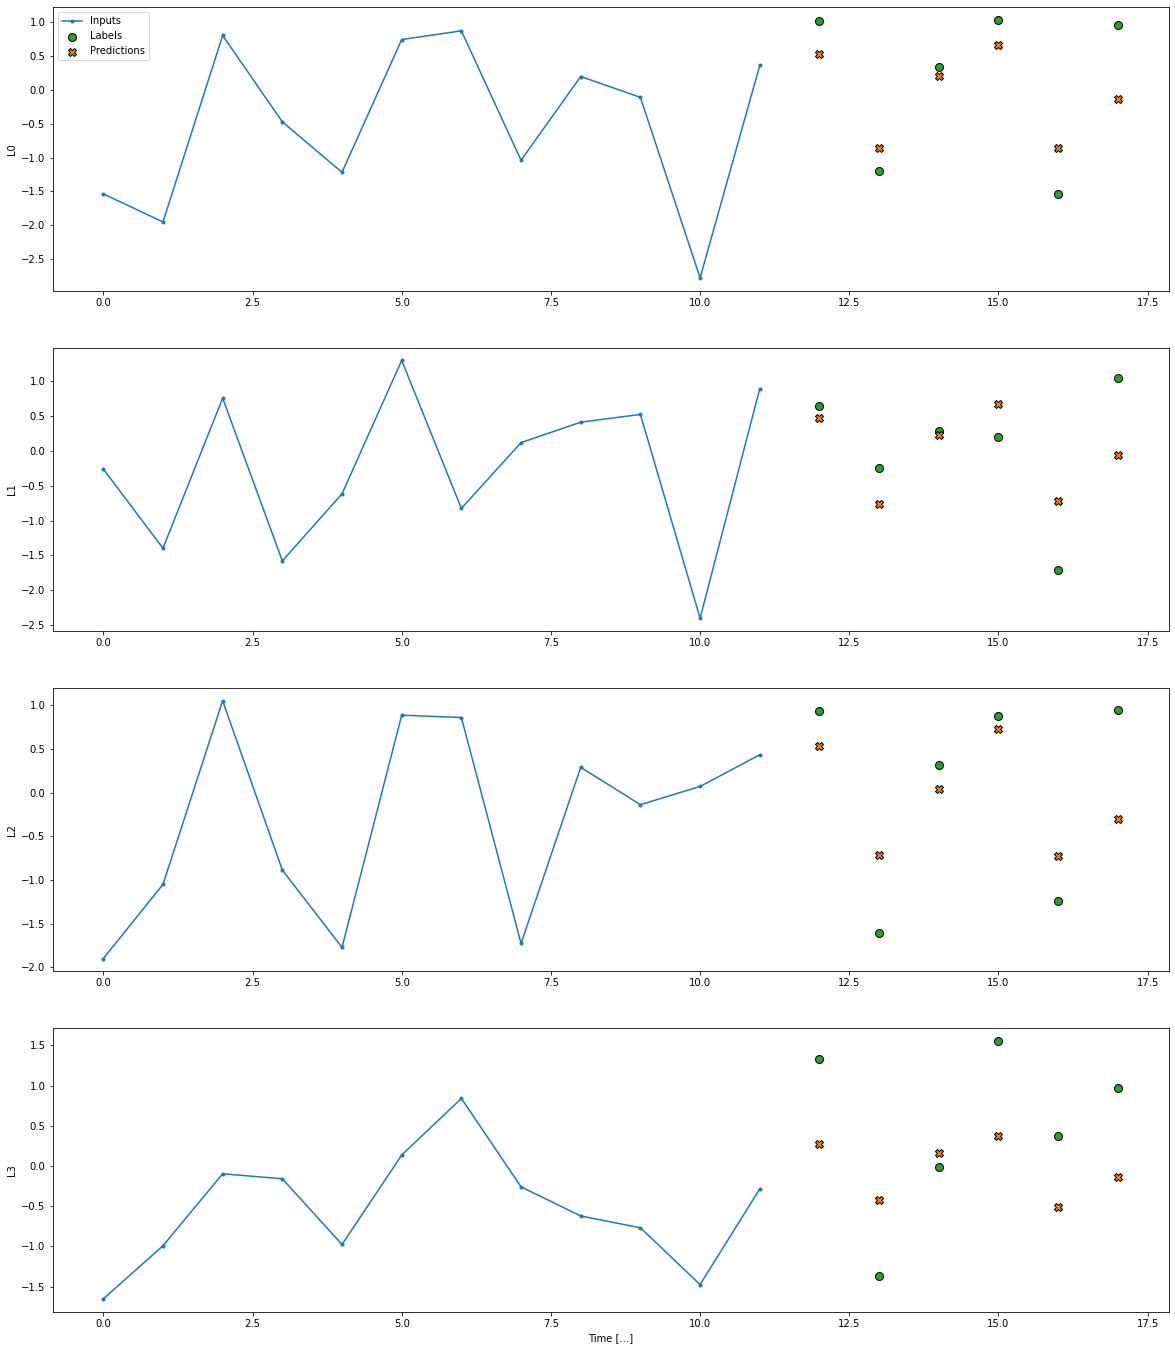
\includegraphics[width=.9\linewidth]{images/GYM-ANM/DATASET PLOTS/lines_forecasting.png}
    \caption[GYM-ANM forecasting]{Forecasting of the values \\
    TODO: denormalise the data for visualisation purposes. Decrease height or split it: too large for this template (it messes up with the layout)}
    \label{fig:net_sit3}
\end{figure}

\noindent The metric used for the evaluation is the mean absolute error (\gls{MAE}):
\begin{algorithmic}
\State $mean\_absolute\_error: 0.6201$
\LineComment{MAE for each feature}
\State $\{L0:0.5625071, L1:0.613873 , L2:0.5569194, L3:0.7471818]$
\end{algorithmic}

\noindent Given this voltage forecast, it would be possible to understand if the network risks overloading for the next time steps and proceed accordingly to avoid damaging the network.



